\cleardoublepage
\markboth{D. ARENA CALIBRATION FIGURES}{}
\chapter{Arena Calibration Figures}

\begin{figure}[H]
\centering
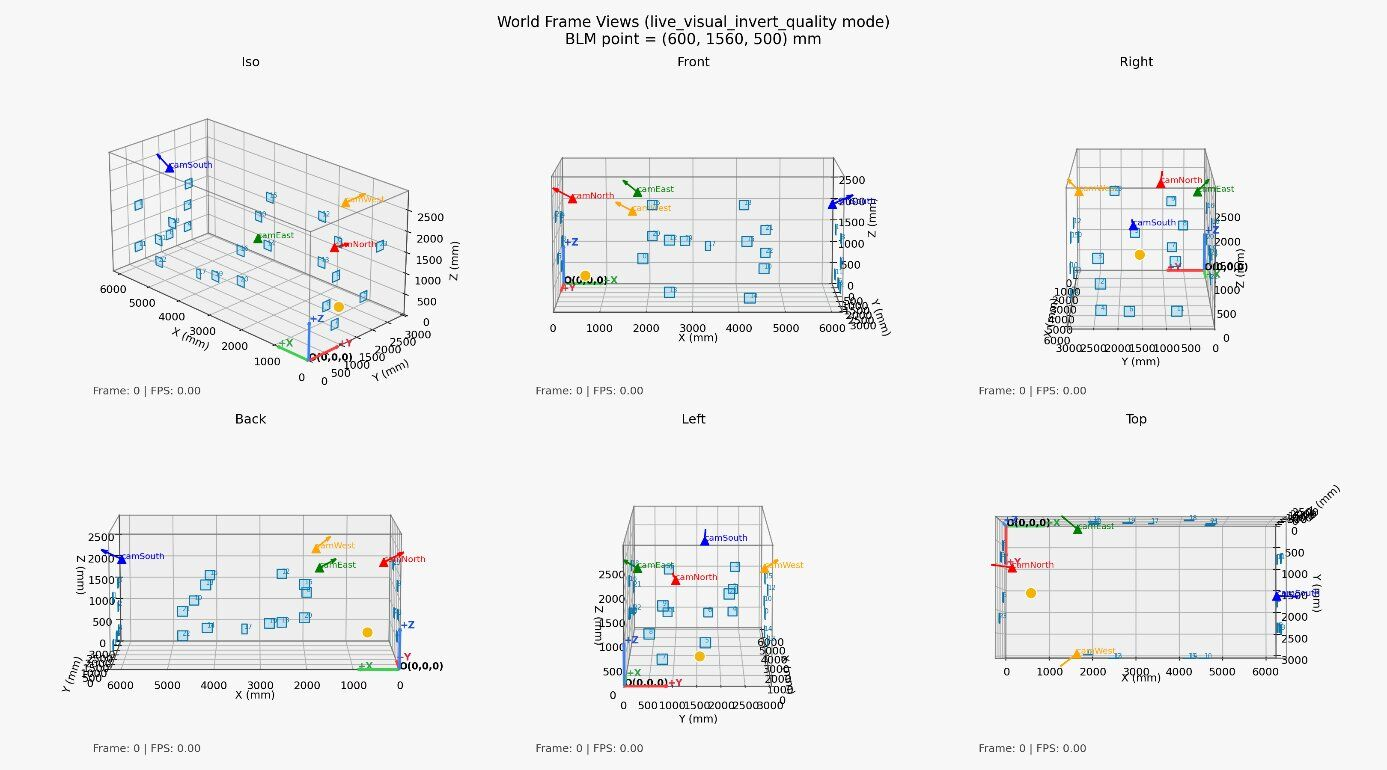
\includegraphics[width=0.9\textwidth]{figures/arena_floorplan}
\caption{\textit{Arena floor plan with camera positions, AprilTag locations, and world-frame axis overlay on all four live camera feeds.}}
\label{fig:d1}
\end{figure}

\begin{figure}[H]
\centering
\begin{subfigure}[t]{0.48\textwidth}
\centering
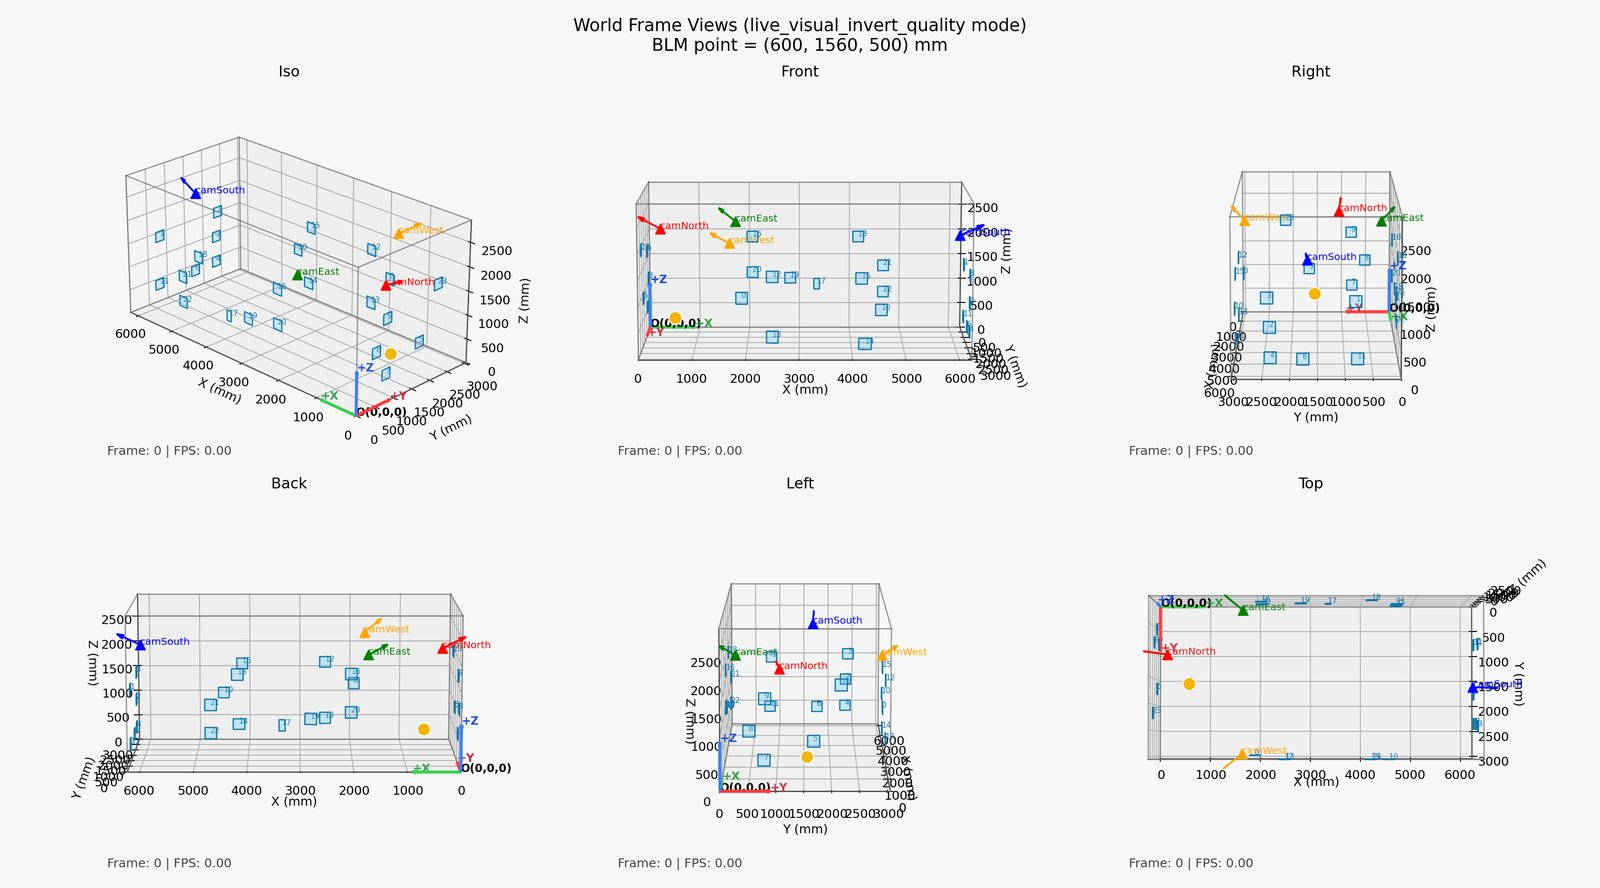
\includegraphics[width=\textwidth,height=0.20\textheight,keepaspectratio]{figures/extrinsic_overlay_cam_a}
\caption*{(a)}
\end{subfigure}
\hfill
\begin{subfigure}[t]{0.48\textwidth}
\centering
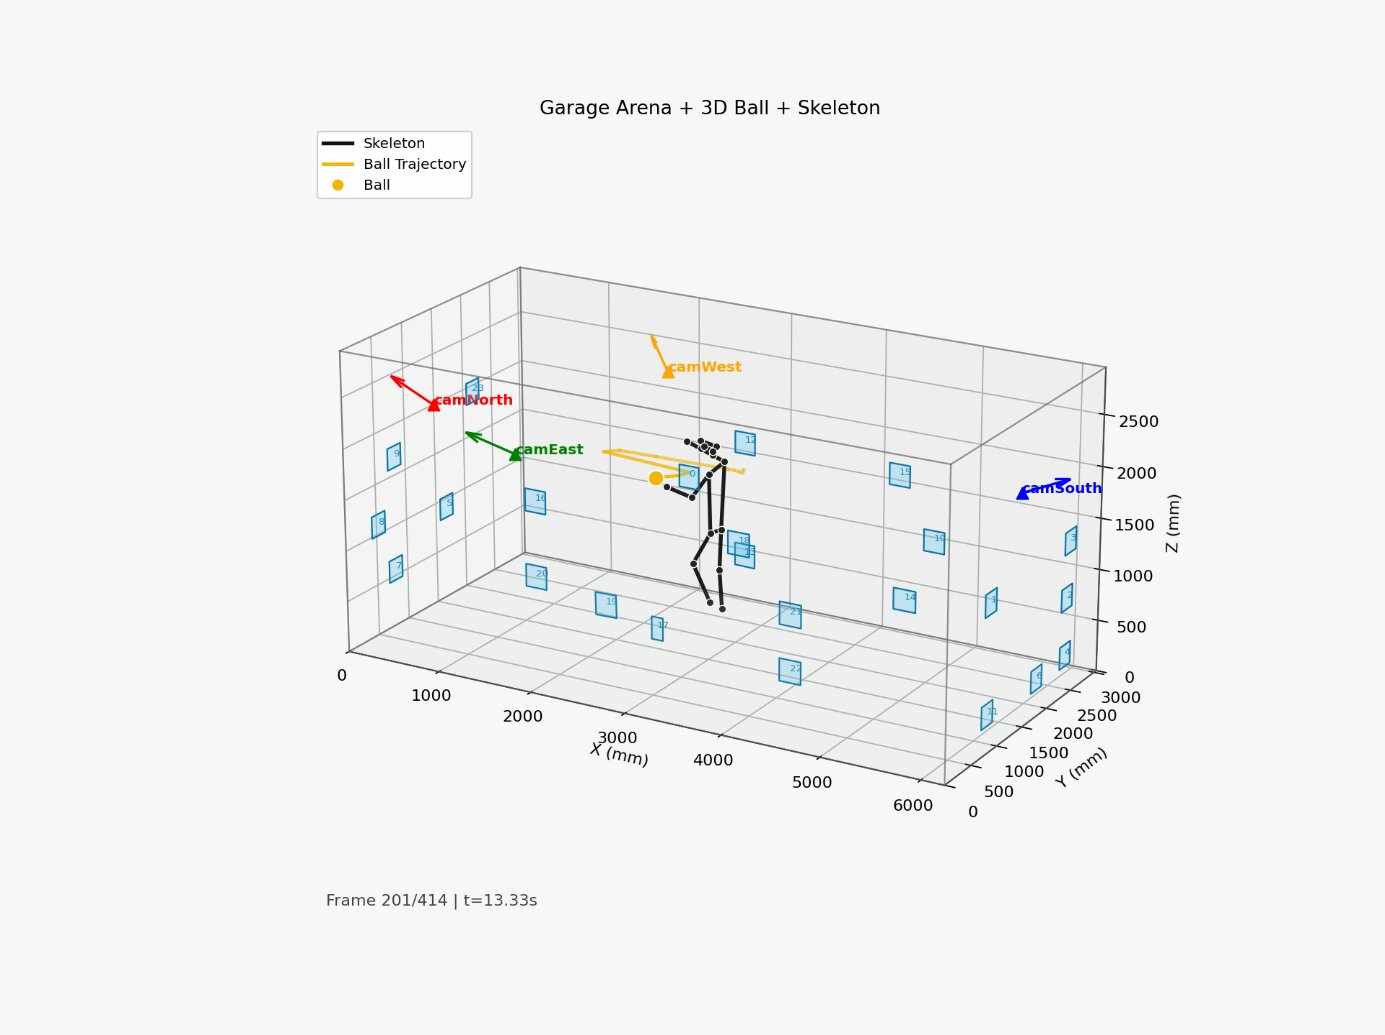
\includegraphics[width=\textwidth,height=0.20\textheight,keepaspectratio]{figures/extrinsic_overlay_cam_b}
\caption*{(b)}
\end{subfigure}

\vspace{0.75em}

\begin{subfigure}[t]{0.48\textwidth}
\centering
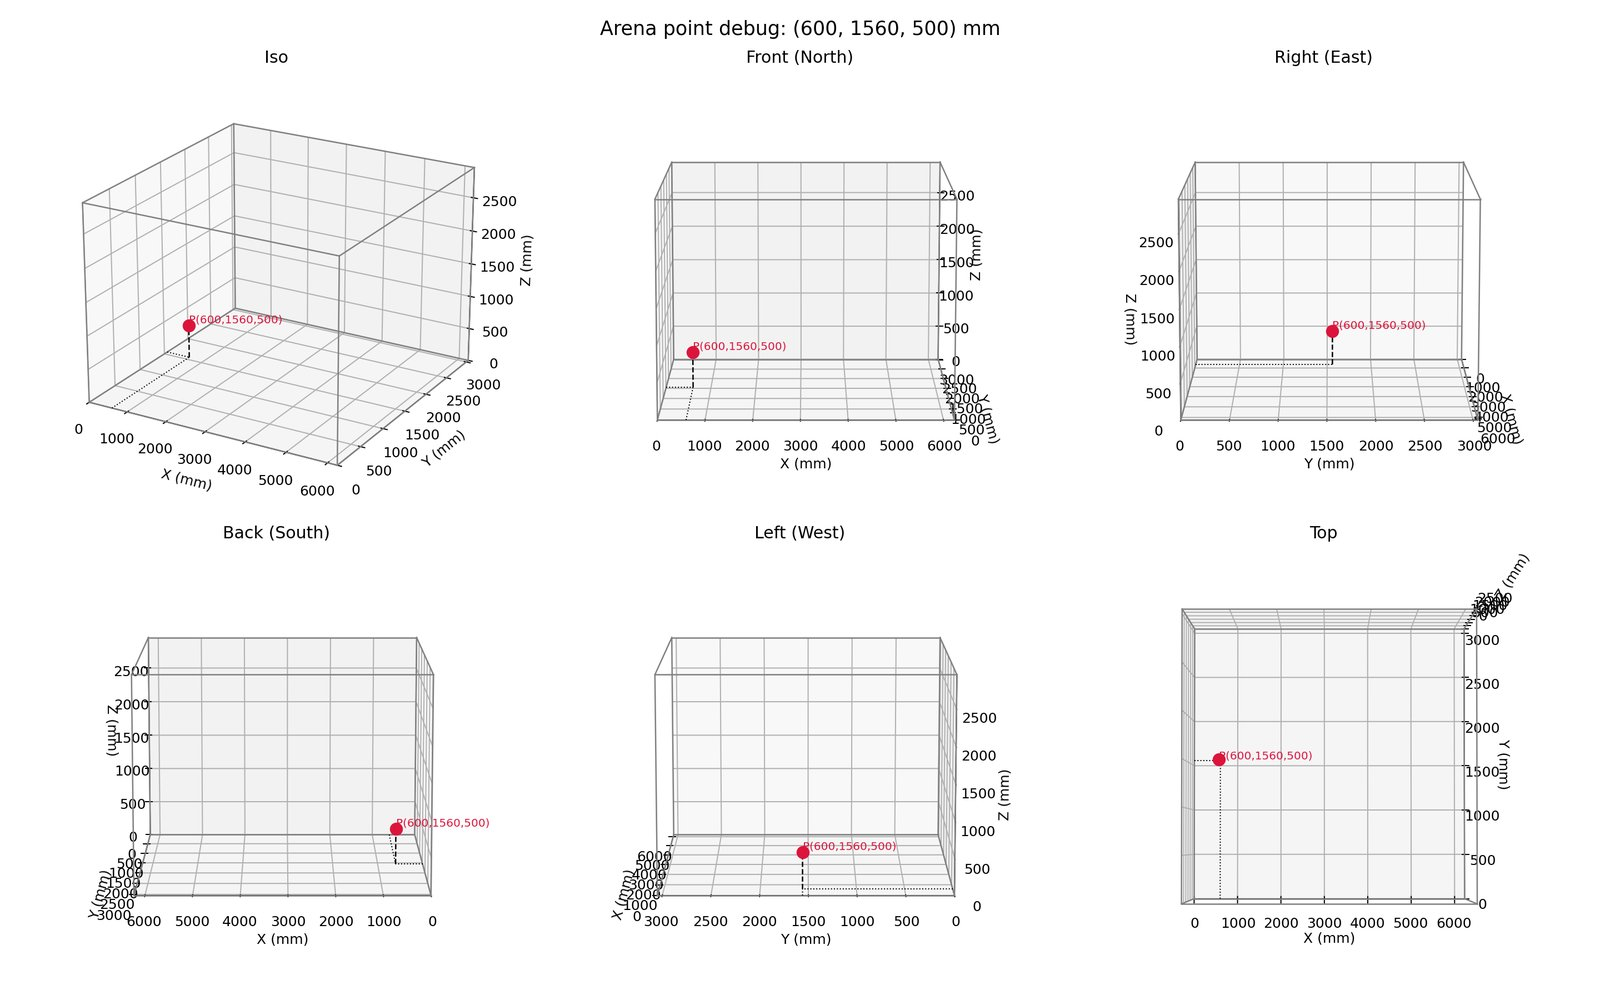
\includegraphics[width=\textwidth,height=0.20\textheight,keepaspectratio]{figures/extrinsic_overlay_cam_c}
\caption*{(c)}
\end{subfigure}
\hfill
\begin{subfigure}[t]{0.48\textwidth}
\centering
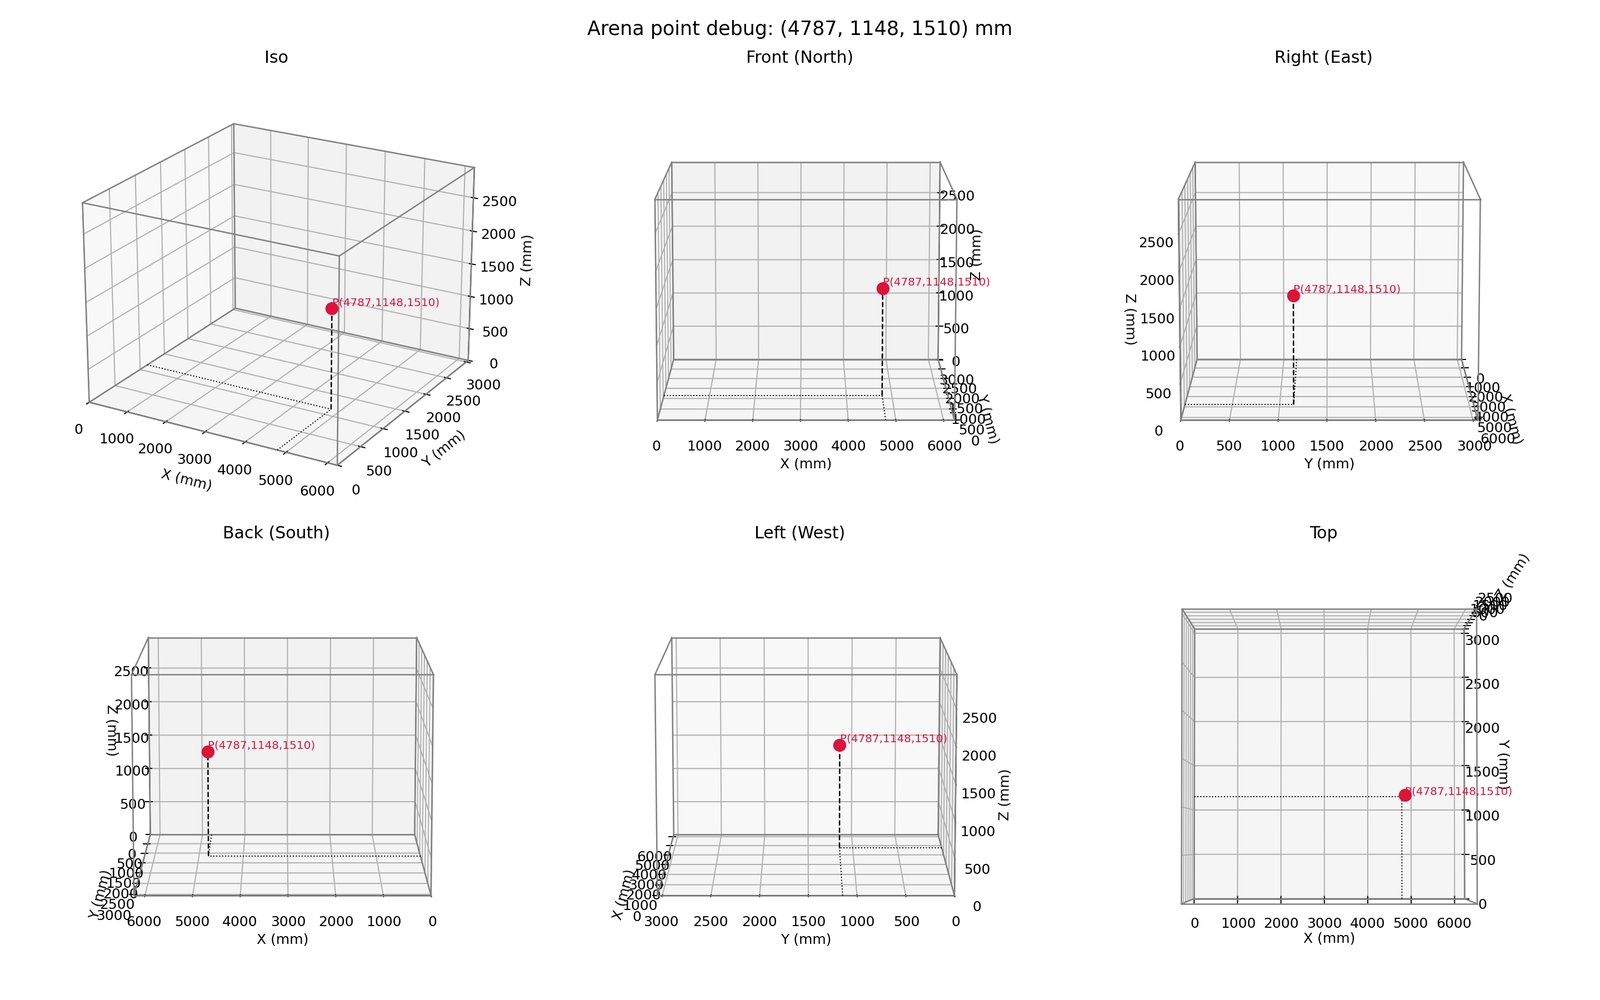
\includegraphics[width=\textwidth,height=0.20\textheight,keepaspectratio]{figures/extrinsic_overlay_cam_d}
\caption*{(d)}
\end{subfigure}
\caption{\textit{Extrinsic overlay validation: reprojected AprilTag corners (red/green markers) overlaid on each camera's live frame, confirming calibration accuracy.}}
\label{fig:d2}
\end{figure}

\begin{figure}[H]
\centering
\begin{subfigure}[t]{0.32\textwidth}
\centering
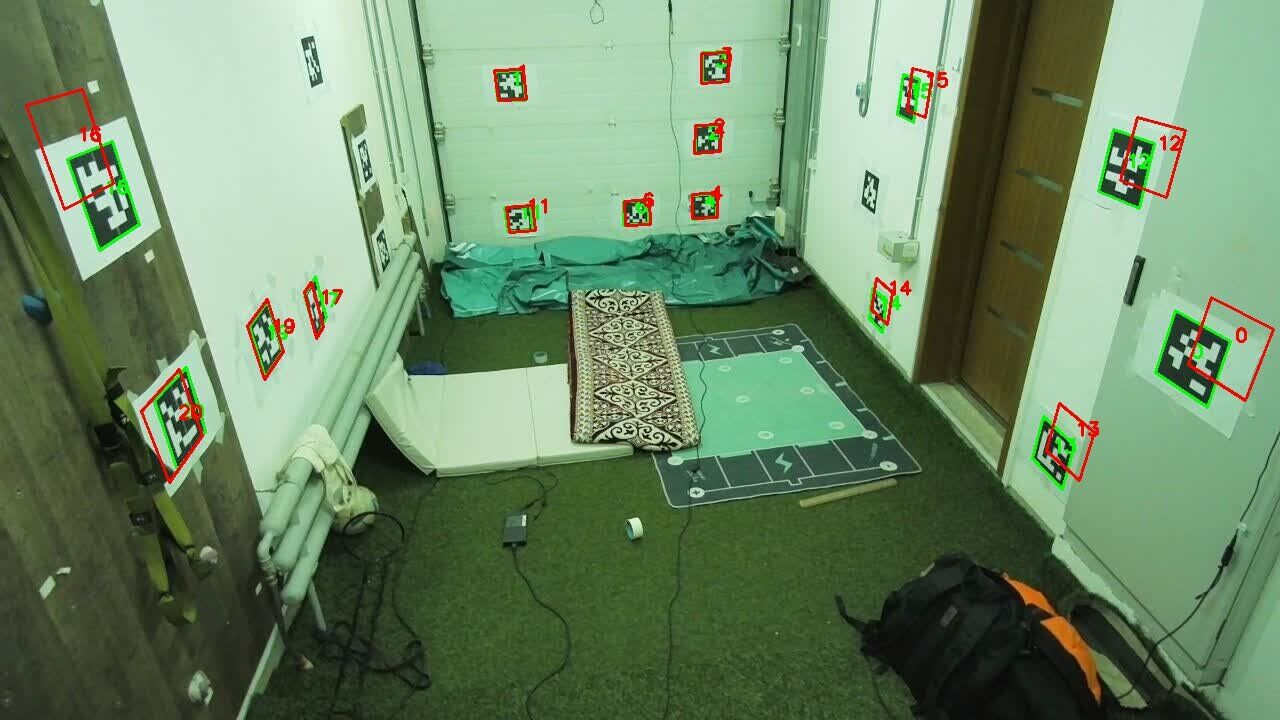
\includegraphics[width=\textwidth]{figures/3d_arena_view_a}
\caption*{(a)}
\end{subfigure}
\hfill
\begin{subfigure}[t]{0.32\textwidth}
\centering
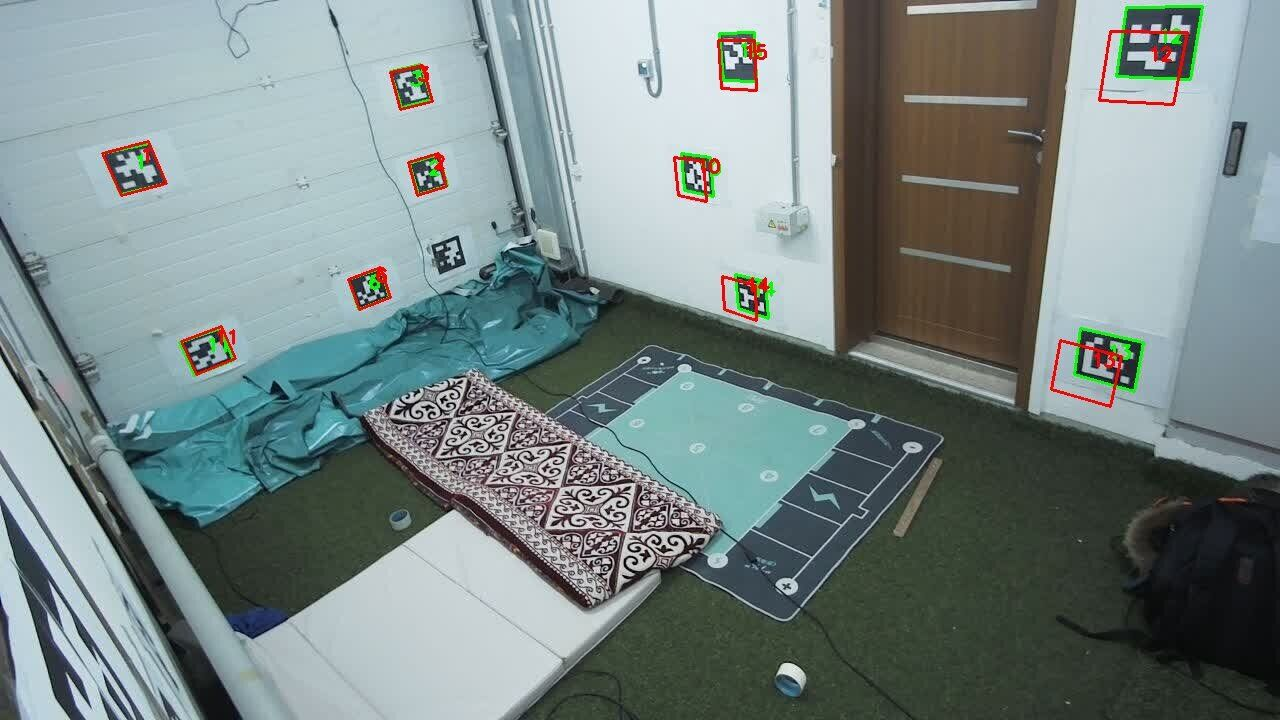
\includegraphics[width=\textwidth]{figures/3d_arena_view_b}
\caption*{(b)}
\end{subfigure}
\hfill
\begin{subfigure}[t]{0.32\textwidth}
\centering
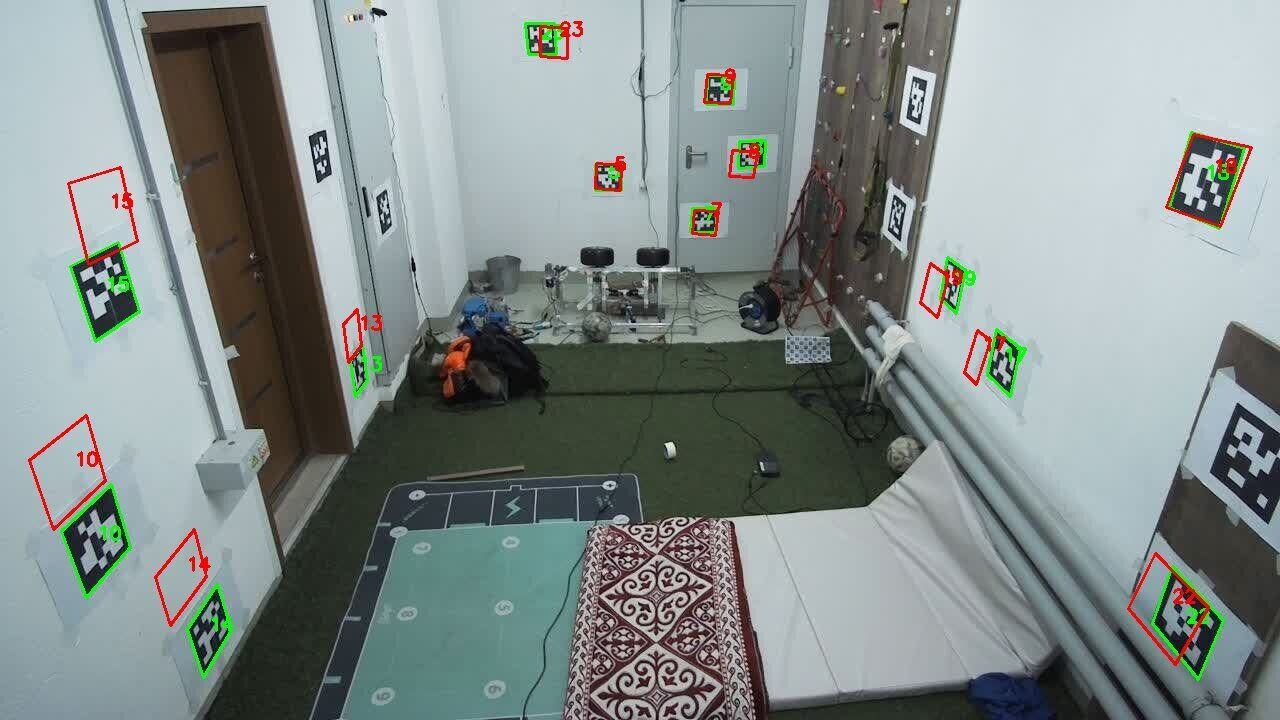
\includegraphics[width=\textwidth]{figures/3d_arena_view_c}
\caption*{(c)}
\end{subfigure}
\caption{\textit{3D arena world-frame renders showing camera positions (coloured markers), BLM position (red), coordinate axes, and AprilTag wall positions from three viewing angles.}}
\label{fig:d3}
\end{figure}

\begin{figure}[H]
\centering
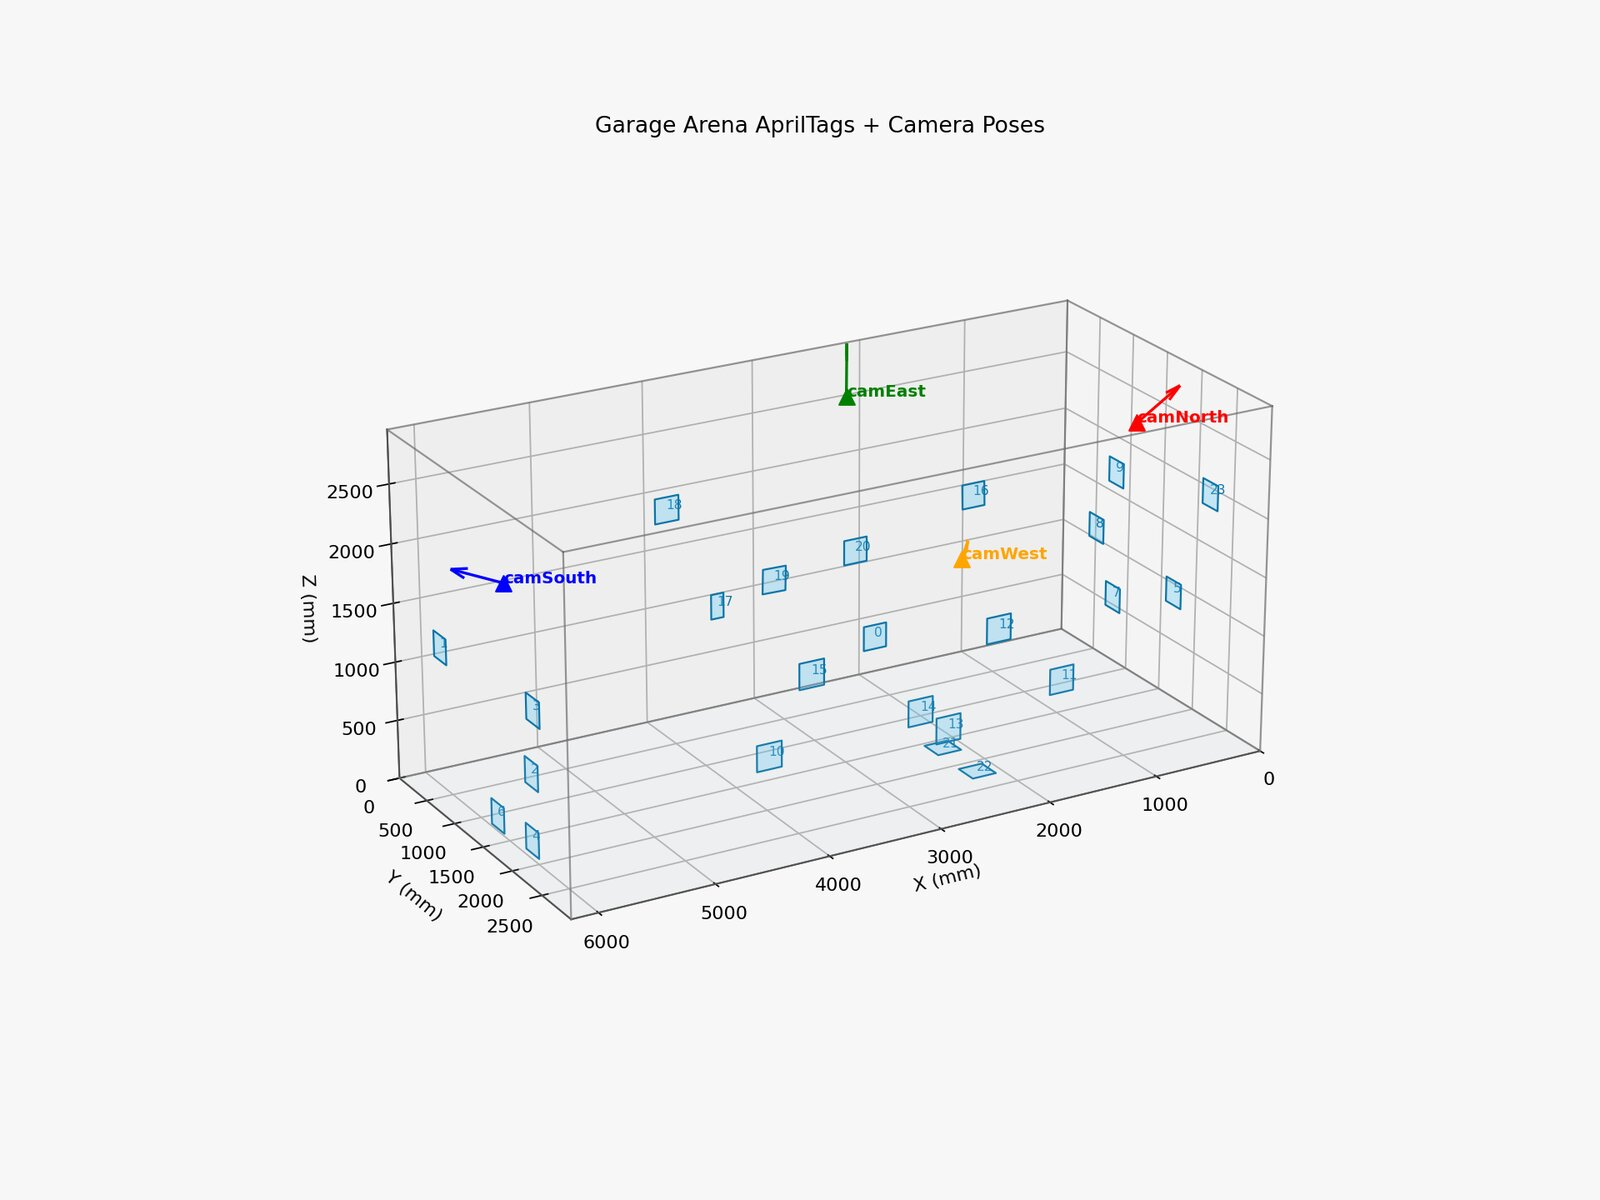
\includegraphics[width=0.6\textwidth]{figures/charuco_board}
\caption{\textit{ChArUco calibration board (A4, 300 dpi, 7 \(\times\) 10 squares, DICT\_4X4\_1000) used for intrinsic calibration of all four cameras.}}
\label{fig:d4}
\end{figure}

\begin{figure}[H]
\centering
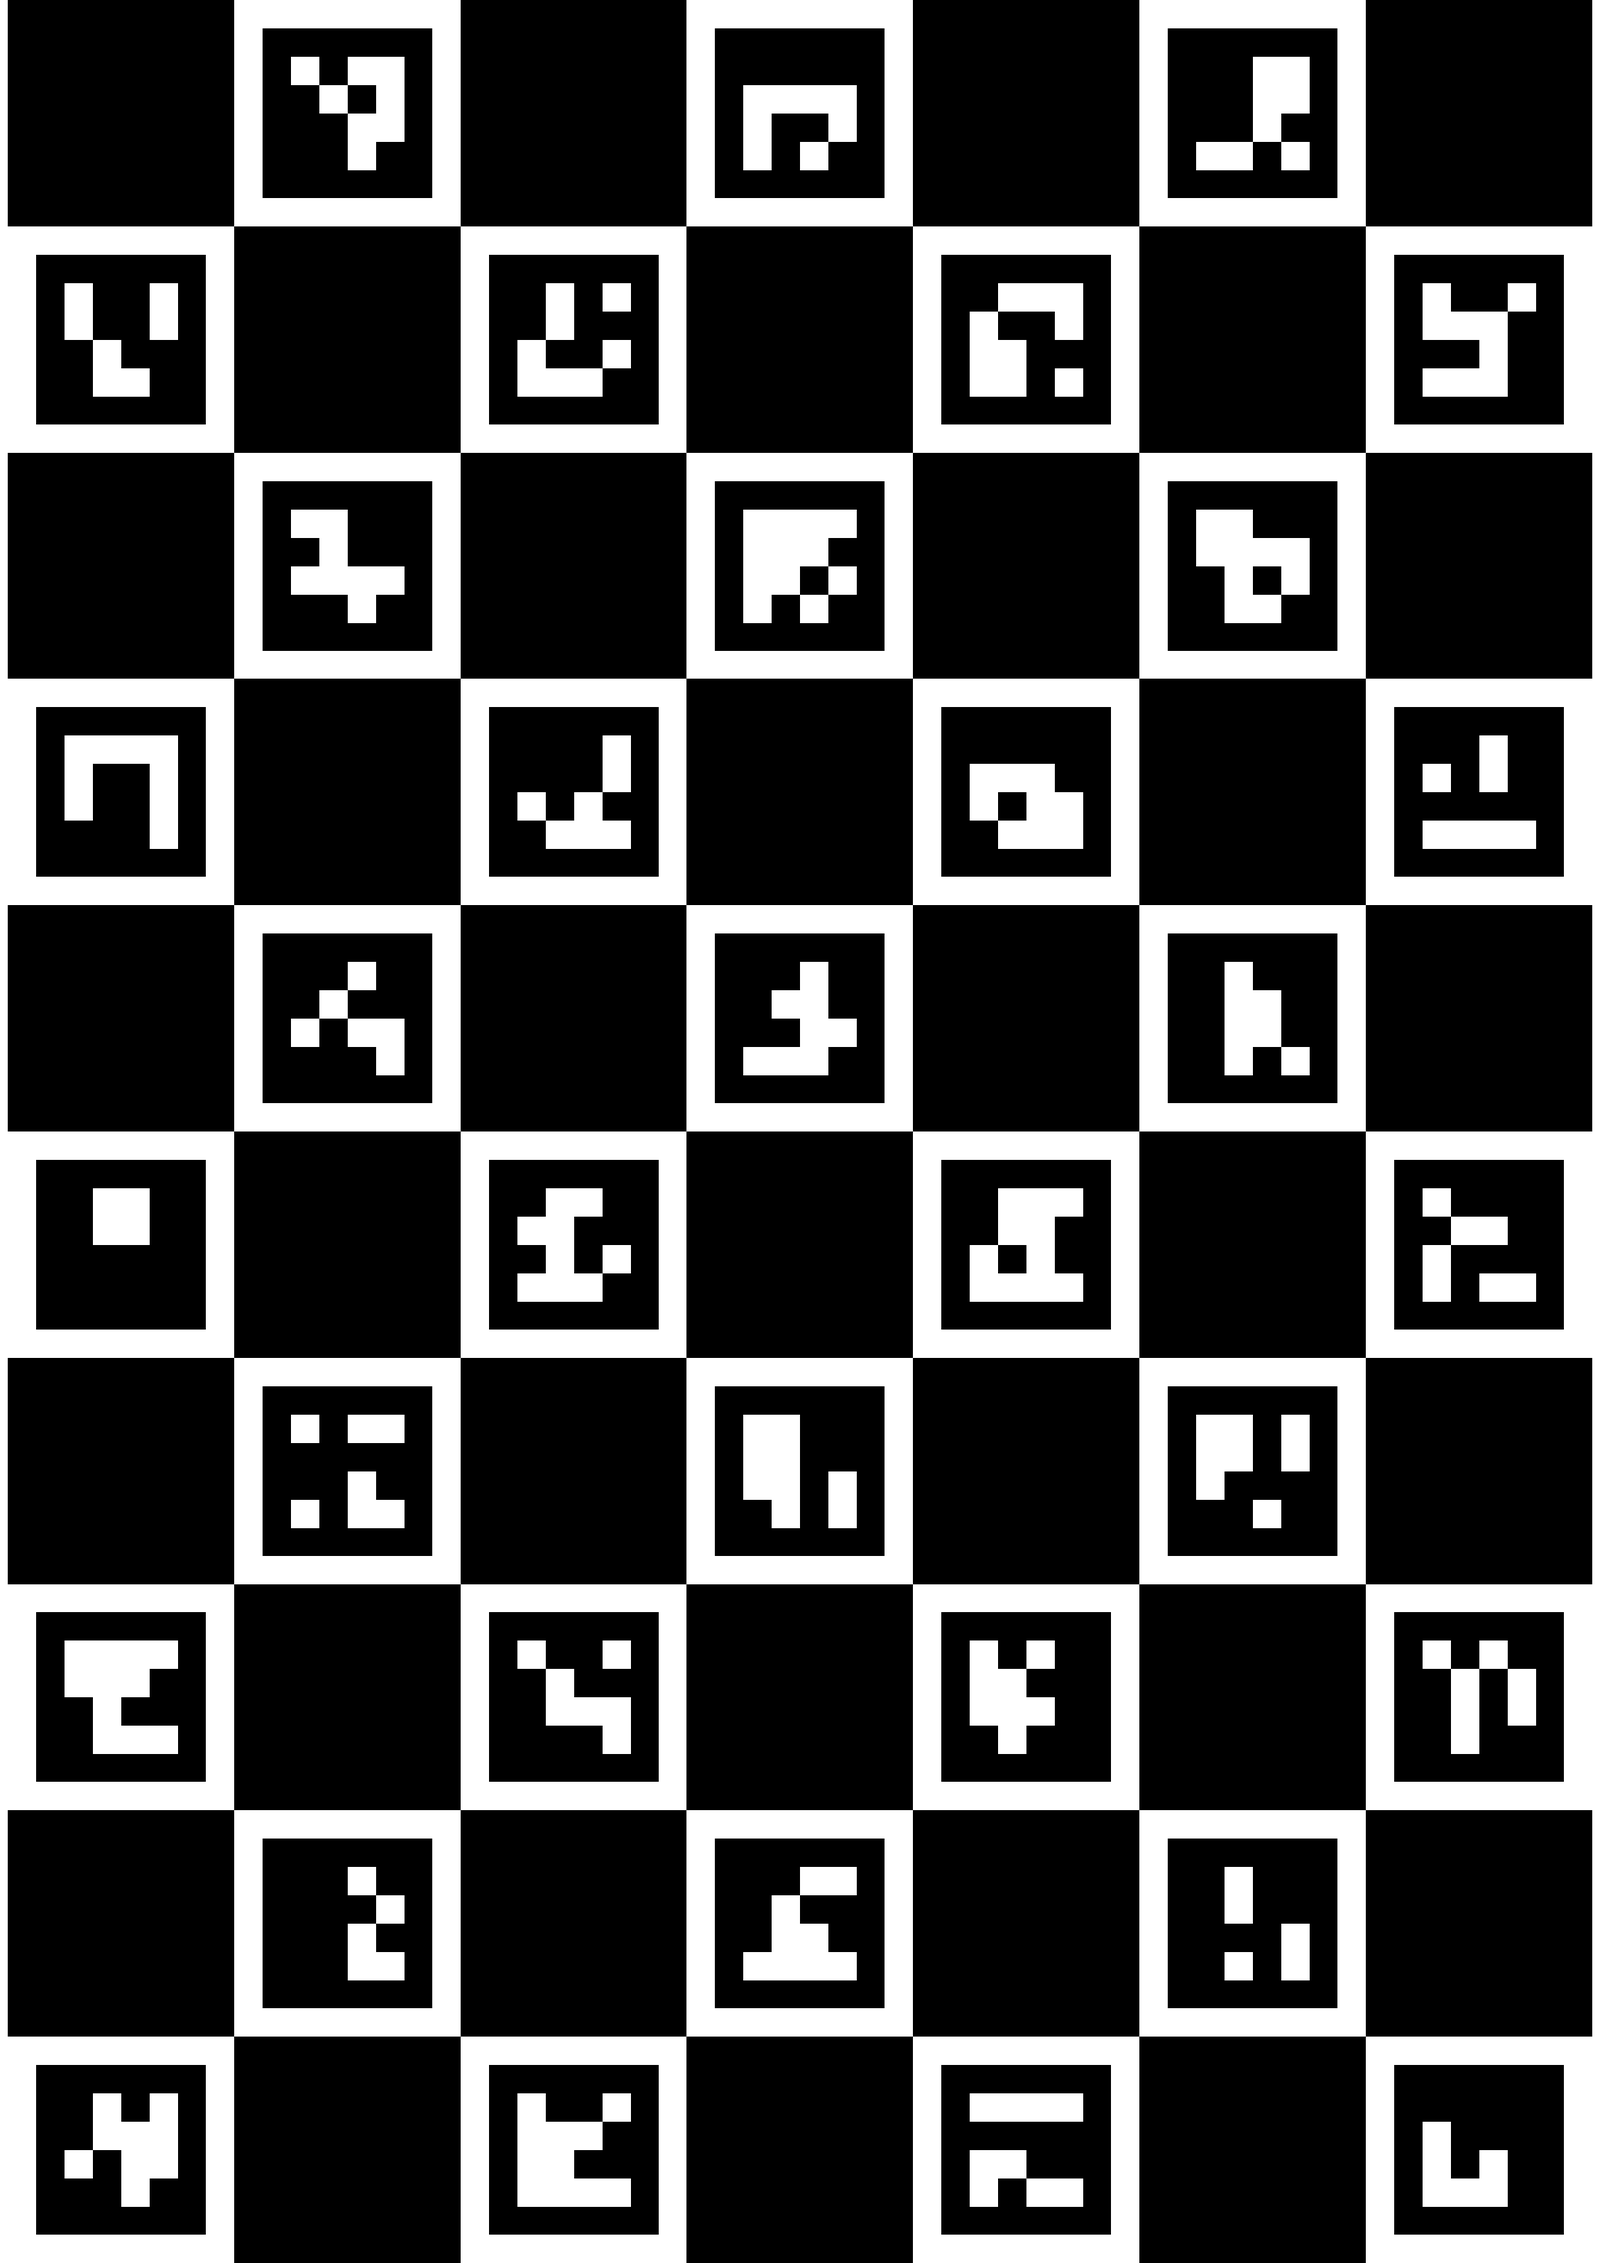
\includegraphics[width=0.75\textwidth]{figures/intrinsic_reprojection_error}
\caption{\textit{Intrinsic calibration reprojection error per camera: bar chart showing per-camera mean reprojection error after ChArUco calibration.}}
\label{fig:d5}
\end{figure}

\begin{figure}[H]
\centering
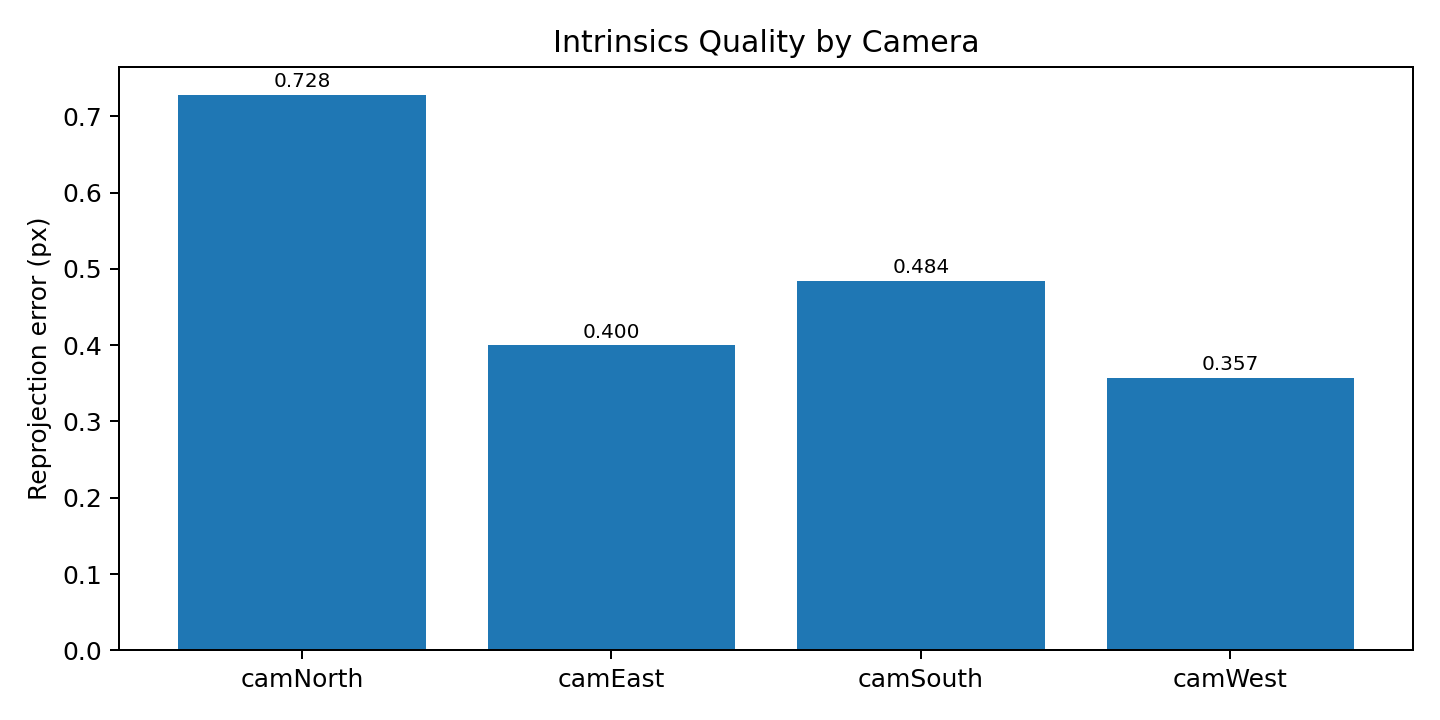
\includegraphics[width=0.75\textwidth]{figures/extrinsic_rmse}
\caption{\textit{Extrinsic calibration RMSE per camera: bar chart showing residual reprojection error after robust PnP optimisation with sigma-clipping.}}
\label{fig:d6}
\end{figure}
